\subsection{Figures}
	\begin{figure}[H]
		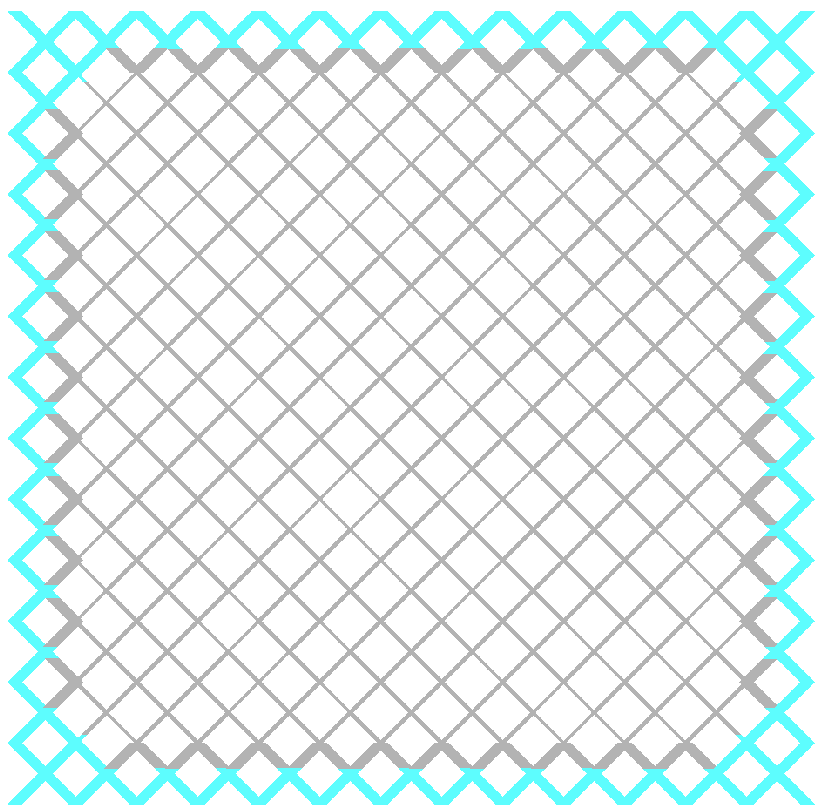
\includegraphics[height=8cm]{fig_result26by26_1}
		\caption{Initial setup}
	\end{figure}
	
	
	\begin{figure}[H]
		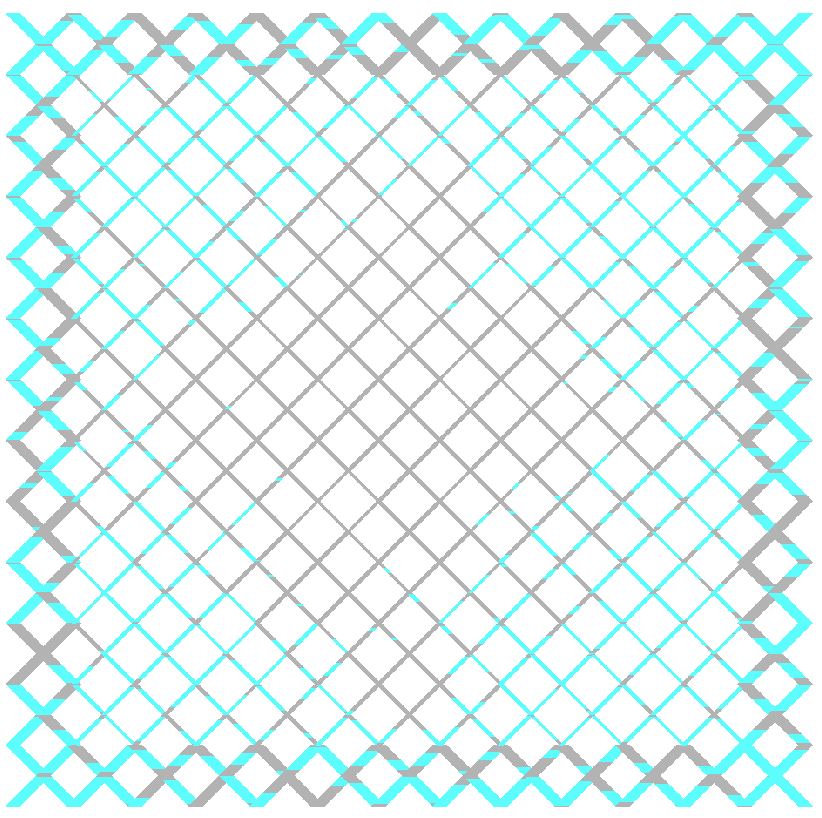
\includegraphics[height=8cm]{fig_result26by26_3}
		\caption{Flow accelerating}
	\end{figure}
	
	\begin{figure}[H]
		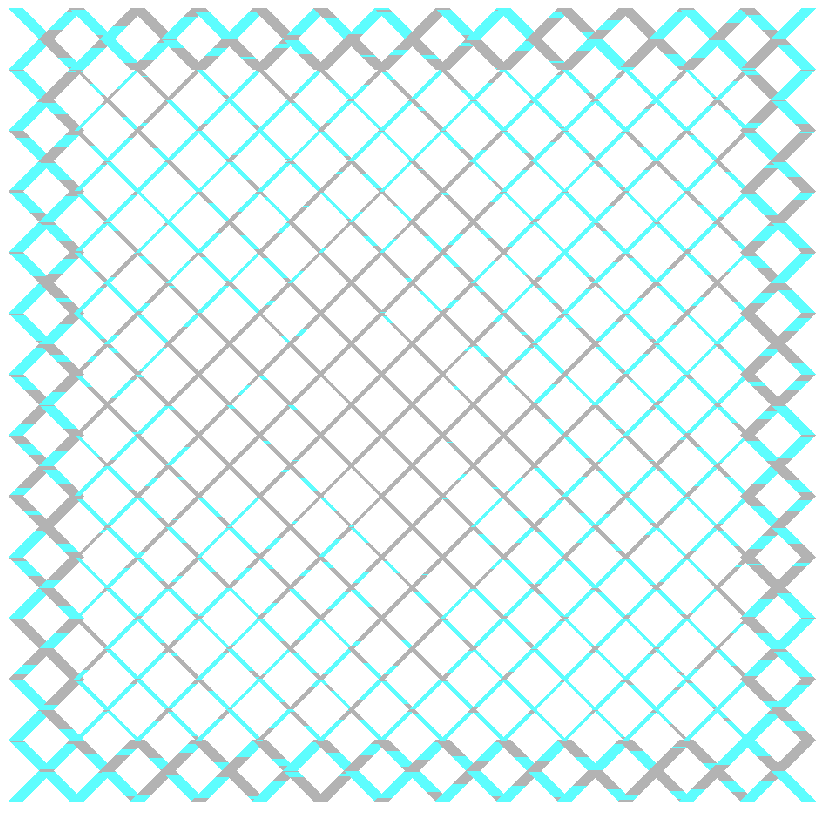
\includegraphics[height=8cm]{fig_result26by26_4}
		\caption{Final}
	\end{figure}

\subsection{Plot}
	\begin{figure}[H]
		\centering
		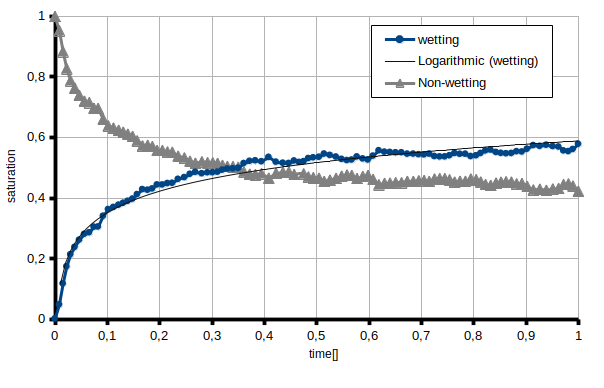
\includegraphics[width=0.8\textwidth]{fig_plot-sat-vs-time2}
		\caption{Plot of saturation of blue fluid in the region of thinner radius with respect to dimensionless time.}
	\end{figure}
	
	Changing the ratio of viscosity affects the rate of displacement in the presence of pressure gradient, however in the case of inbibition significant differences were not observed.
	
\subsection{Discussion}
	\begin{enumerate}
		\item Calculation was done for 20,000 steps.
		\item Plot for every 200 frames.
		\item Equal volumes of each phases.
		\item The saturation for wetting fluid is $0.57$ for the inner region, which is very close the previous simulation for 10x10. 
		\item It is clear that the relaxation parameter is present as the saturation converges to an equilibrium value.
		\item For the simulations the length of each tube was taken to be unity and only the ratio of viscosity was used in equation \ref{eq:flow-rate-main}, since these values do not change the geometry of the flow and change only the scale of time. Dimensionless value of time was used.
		\item Logarithmic dependence was observed [EDIT-ADD equations determine the physical meaning of the non equilibrium parameter, and the scope of its applicability.]
	\end{enumerate}
		

		
		
	
